\chapter{Methods}
\label{sec:methods}

\section{Survey}
\label{sec:survey}
To begin exploring how securely local inter-process communication is used, I first needed to find out what applications use local IPC resources.  To do so, I created a survey that would gather information about what processes were currently running on a computer and what local IPC resources each consumes.  The goal of this survey was to find out how many computers each application was running on and which applications used the most of each form of local IPC.  Using this data, I could make an informed decision about which applications to look into and find applications that I would be able to fuzz effectively.  This meant finding applications that used many local IPC resources and specifically many named UNIX domain sockets as opposed to \texttt{socketpair} sockets.

The survey is made up of a shell script that makes each observation and outputs the data to files, in addition to two Python scripts which were used to anonymize the data and find the process and user owning the other end of UNIX domain sockets, pipes, and FIFOs.  This survey gathered information about all open pipes, named pipes, UNIX domain sockets, TCP sockets, and UDP sockets.  The tool used to find this information is called \texttt{lsof} which stands for list open files.  I sent the survey to over 250 people to run on their computers and received 22 responses, representing roughly an 8.5\% response rate.  The survey ran on each person's computer, taking observations roughly over a two day period.  

\begin{figure}
\centering
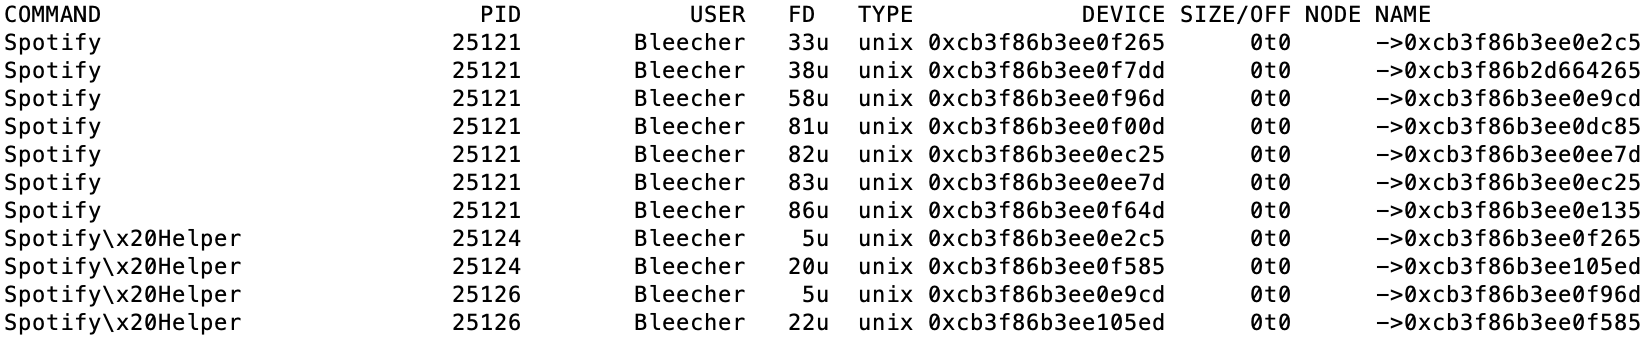
\includegraphics[width=1\textwidth]{lsofOutput.png}
\caption{Sample of \texttt{lsof} Output for UNIX Domain Sockets}
\label{fig:lsofOutput}
\end{figure}

The script collected eleven files per computer.  One file contained the anonymized output of the \texttt{ps} command, which describes all of the processes currently running on the machine.  This data is used to connect processes together under the umbrella of the application they work for.  These are often called helper processes since they work to help the main process function.  I also collected the anonymized raw output of \texttt{lsof} after filtering for a specific type of local IPC.  Therefore, there are five files containing this data, one each for anonymous pipes, named pipes, UNIX domain sockets, TCP sockets and UDP sockets.  An example of this is shown in Figure~\ref{fig:lsofOutput} which shows the \texttt{lsof} output for UNIX domain sockets filtered to look just at \texttt{Spotify}.  In addition, for each of these types of local IPC, there is another file that represents how many of each type a process has open at one time.  For example, instead of six lines showing the different UNIX domain sockets that \texttt{Spotify} has open at one time, one observation in this file would have the process name, \texttt{Spotify}, and the number of local sockets, 6, without any of the other information outputted by \texttt{lsof}.  Figure~\ref{fig:countOutput} gives a piece of one of these count files.  All of these files were uploaded to the Middlebury College Computer Science Department's machine, basin.

\begin{figure}
\centering
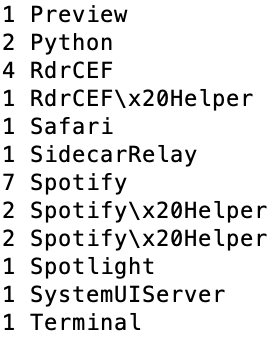
\includegraphics[width=0.25\textwidth]{countOutput.png}
\caption{Sample of a count file for UNIX Domain Sockets}
\label{fig:countOutput}
\end{figure}

All identifying information was anonymized so that no data can be attributed to any individual.  To remove all username mentions, I used the \texttt{dscl} utility to find a list of all users on the computer.  I removed some users from this list such as \texttt{root}, \texttt{nobody}, and \texttt{Guest} who did not need to be anonymized.  Then, for each file that could possibly contain a username, I ran a Python script that replaced each occurence of a listed username with USERNAME.  This is shown in Figure~\ref{fig:lsofAnon} which has the \texttt{lsof} output where the username has been replaced.  In doing this, I lost the ability to differentiate between different user accounts on a single computer, but it is unlikely that different human users were running applications since all computers were personal computers.  I was, however, able to tell between a human user and either \texttt{root} or another automated account, such as \texttt{\_mDNSResponder}.

\begin{figure}
\centering
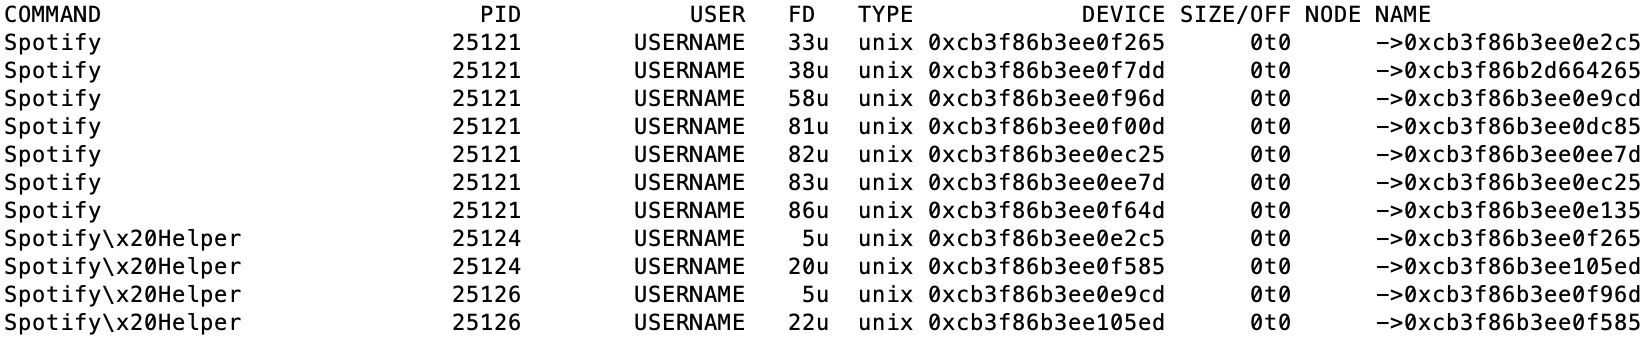
\includegraphics[width=1\textwidth]{lsofAnon.png}
\caption{Sample of Anonymized \texttt{lsof} Output}
\label{fig:lsofAnon}
\end{figure}

I also wanted to be able to see if connections were being made between processes running under different users, specifically between a normal user and \texttt{root}.  I made another Python script that found this information for UNIX domain sockets, pipes, and named pipes.  First, for each individual end of a UNIX socket, pipe, or FIFO, it found the user owning that end and the device number corresponding to it.  Then, it looked in the column representing the other end of the communication, and matched the process and user that was on the other end.  This way, I could see which users and processes were communicating with each other.  Figure~\ref{fig:lsofConn} shows a sample of this output.

\begin{figure}
\centering
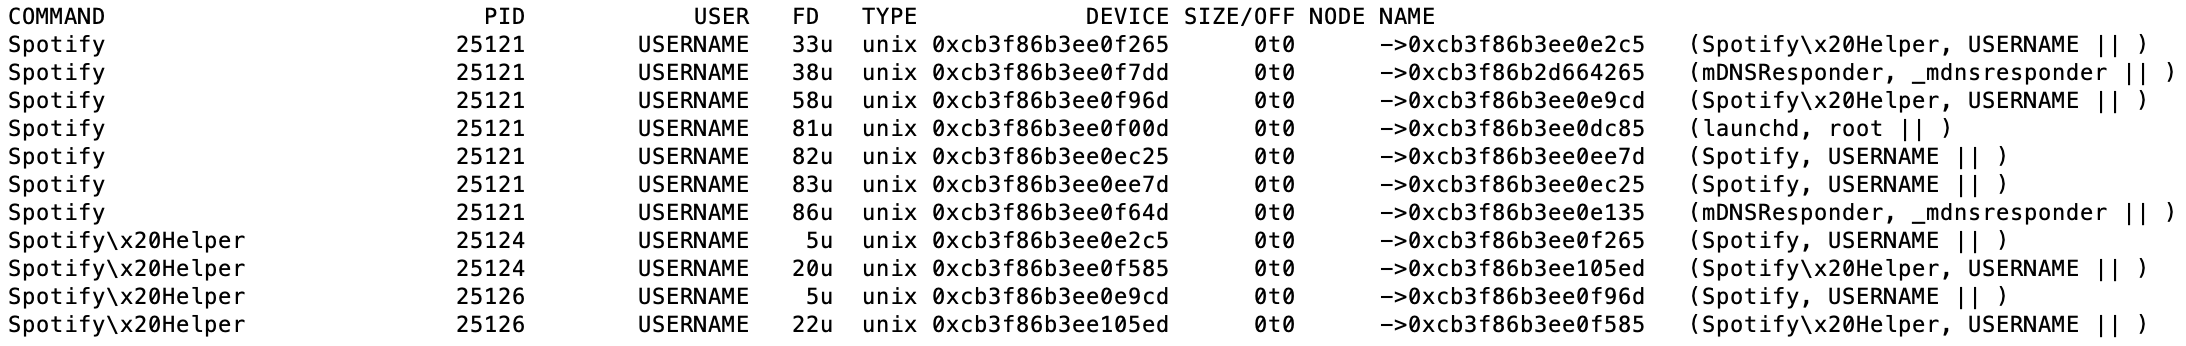
\includegraphics[width=1\textwidth]{lsofConn.png}
\caption{Sample of Anonymized \texttt{lsof} Output with Connections}
\label{fig:lsofConn}
\end{figure}

\section{Extracting Results}
\label{sec:extractResults}
Once I had all of the data, I created another Python script to extract the results to inform my decision of what applications to look into.  First, I  looked through all of the processes that were running and manually created groups of processes that were part of the same applications.  For some, like \texttt{Spotify} and \texttt{Spotify Helper}, it was easy to tell that both processes are part of the application \texttt{Spotify}.  However, for others, like \texttt{Safari} and \texttt{com.apple.Webkit.Networking}, I had to research each process on Google to find out that these processes both were part of the \texttt{Safari} application.  A complete list of these groups is provided in Appendix~\ref{appendix:processGroups}.

Then, I created a table that contained the results for every application I manually recognized, or for each process if I did not assign it to a particular application.  For each application, the data table contains the name of the application, the number of different computers that had this application running at least once, and the average number of named pipes, anonymous pipes, local and total TCP and UDP sockets, and UNIX domain sockets open at any time.  It also contains all of the users that had at least one end of a communication channel with that application.

This data, particularly the average number of open FIFOs, local TCP and UDP sockets, and UNIX sockets, was what I used to decide what applications were the most important to examine.  Another important aspect which is not reflected in this table was whether an application's UNIX socket was named.  This was important because I cannot connect to an unnamed UNIX socket, created through the \texttt{socketpair} system call, without explicitly being given an endpoint.  Therefore, if an application had UNIX sockets and at least one was named in the filesystem, then I was more likely to choose this application because I would be able to fuzz it and generate results, unlike the \texttt{socketpair} sockets that I could not fuzz at all.

\section{Fuzzing}
\label{sec:fuzzingMethods}
As described in Section~\ref{sec:fuzzing}, fuzzing is the process of sending random or semi-random data to a communication endpoint in an attempt to explore how the receiving process deals with unexpected input.  I decided to use \textit{radamsa}~\cite{radamsa} for my fuzzing software.  I chose \textit{radamsa} for a variety of reasons.  First, it is an easy-to-install fuzzer.  Because of the short timeframe I have for this thesis, I needed a high-quality fuzzer that would not take long to tune or understand how it works.  \textit{radamsa} provides just that.  All that is needed is to douwnload the source code and compile it, and the resulting executable is all that is required to successfully fuzz.

The second reason that I chose \textit{radamsa} is because it has no frills.  All that \textit{radamsa} does is take valid input and randomly modify it.  There is no fancy interface to use and more importantly, no parameters to tune.  I send a valid example of a message as input and an altered string is returned.  This message can then be encapsulated within the packaging required to send the data over the desired communication channel.  This allows \textit{radamsa} to easily be included in a script that generates semi-random input, sends it to the tested endpoint and checks to make sure that the program is still running.  That is exactly what I did.

\section{Seeing Local IPC Communication}
\label{sec:seeingLocalIPC}
To make my fuzzing more effective, I needed to find examples of genuine messages being sent to the open sockets and named pipes that I was planning on fuzzing.  To do this, I needed to see what messages were being sent.  For communication over the loopback interface, this was simple.  I downloaded and installed \textit{Wireshark}, an application that shows the raw bytes being sent through different network interfaces and identifies the different headers from each layer when it is able to understand a packet.  This way, I was able to see every bit of every message that went through the loopback interface.

Named pipes and UNIX domain sockets did not have a similar, easy way to view all messages.  Once I found the name of a named pipe in the filesystem, I could join the pipe as a reader.  However, I would not see every message sent through the pipe if there were other readers.  Each message is only received by a single reader.  Therefore, if I was one of many readers, the single process that was given a message was randomly selected.  Neither the privilege level of the user running the pipe reader nor the order in which the processes started reading from the pipe affected which process received the message.

If the named pipe was not random, then I could delete the pipe from the filesystem and create a new one with the same name.  I did this to see what messages were being sent from the clients to the server.  This would give me messages that I could modify to fuzz the servers.  Since most communication follows the request/response pattern, I captured most of my sample messages by impersonating the server and capturing these genuine requests.

Communication over UNIX domain sockets is even more difficult to observe than named pipes.  For sockets that are created by \texttt{socketpair}, it is impossible to view their data without being explicitly given an endpoint.  I could not get any of these endpoints in my testing, so these messages were completely hidden from my view.  However, it is sometimes possible to view data sent through a named UNIX domain socket.  Like Internet sockets, UNIX domain sockets know information about the other side of the communication, and can create separate communication channels.  For example, for stream sockets, each connection that a listening socket accepts is separate from one another.  The server is able to differentiate between the different clients, and messages sent to one connection are not sent to all others.  Therefore, to receive messages from the clients, one must create the listening UNIX domain socket before the true application does.  Receiving messages from the server is more difficult, because I had to connect to the server and send messages that elicit a response.  Essentially, I needed to fuzz the server without any data to base the packets on and hope that one of the random packets get a response.

In the next chapter, I will go into more depth on how I found sample messages for different forms of local IPC for the applications that I studied.  I will also discuss the fuzzing and other tests I ran to find how secure these communications are.
